%
%  $Description: Author guidelines and sample document in LaTeX 2.09$
%
%  $Author: mankit $
%  $Date: 2008/05/20 07:24:15 $
%  $Revision: 1.41 $
%

\documentclass[times, 10pt,twocolumn]{article}
\usepackage{latex8}
\usepackage{times}
\usepackage{amssymb}
\usepackage{amsmath}
\usepackage{stmaryrd}
\usepackage{graphicx}
\usepackage{fancyvrb}
\usepackage{color}
\usepackage[small]{caption}
\usepackage{sidecap}
%\documentstyle[times,art10,twocolumn,lat ex8]{article}

%-------------------------------------------------------------------------
% take the % away on next line to produce the final camera-ready version
%\pagestyle{empty}

%-------------------------------------------------------------------------
\begin{document}

  \title{Elimination of Timing Attacks with a Precision Timed Architecture}

  \author{Isaac Liu, David McGrogan \\
    Center for Hybrid and Embedded Software Systems, EECS \\
    University of California, Berkeley \\
    Berkeley, CA 94720, USA \\
    \{\tt liuisaac, dpmcgrog\}@eecs.berkeley.edu
  }


\maketitle
\thispagestyle{empty}

\begin{abstract}
Side-channel attacks exploit information-leaky implementations of cryptographic algorithms to find the encryption key. These information leaks are caused by the underlying execution platform which contain hardware elements designed to optimize performance at the expense of predictable execution time. This shows that for security systems, not only does the software need to be secure, but the execution platform also needs to be secure in order for the entire system to be truly secure. PRET is an architecture designed for real time systems that has total predictability without sacrificing performance. It contains ISA extensions to bring control over temporal properties of a program to the software level. We show that this design can not only defend against all software side channel attacks on encryption algorithms, but completely eliminate the root cause of the problem. We demonstrate this by running a reference implementation of the RSA algorithm on PRET and prove that it's immune to side channel attacks.
\end{abstract}

%encryption info
%	explain a little about the applications of encryption and how it works
%- side channel attack info
%	brief summary on side channel attacks, including timing, cache, branch predictor (i can add this in later), and maybe even power
%- Pret
%	Explanation of the architecture, and deadline instruction (you can take some graphics off our paper or the current poster template)
%-source code
%	I'll add in some source code snap shots of how to program with deadlines
%-Results
%	Plots of data and timing information

%\section{Outline and Breakdown}
%\begin{itemize}
%\item abstract, Introduction  - Isaac
%\item Related Work - David
%\item Encryption and Side Channel Attacks - David
%\item PRET  - Isaac 
%\item Results  - Isaac
%\item Conclusion and future work - David
%\end{itemize}

%------------------------------------------------------------------------------
\section{Introduction}
Encryption is at the heart of every security system. By scrambling sensitive messages with a key, private information is kept private because even if the message is intercepted, the advisory has cannot retrieve the contents of the message. This is basis for authentication servers, secure connections and many more. A good encryption algorithm contains strong mathematical properties that even if the advisory knows the encryption algorithm and eavesdrops on the encrypted message, it will still be nearly impossible with the computing power today to decode the message without the key.

However, attackers soon realized that instead of directly attacking the mathematical properties of the algorithm, they can instead infer information from the underlying implementation, and gain a huge advantage in obtaining the key. These attacks are called side channel attacks. Timing channel attacks use run time variances of encryption algorithms to retrieve the keys. Branch predictor attacks use information from the hardware branch predictor to follow control flow of the encryption algorithms, gaining insight of the key. Cache attacks use information from the caches and observe the data accessed in the encryption algorithm to derive the key. All these attacks target the unpredictable and uncontrollable temporal properties of the underlying architecture, which the software has no control over.  It may be true that special coding techniques can mitigate the chance of success for some specific attacks, but the root vulnerability is still present, which is the uncontrollable temporal semantics of the architecture. Any other security software will still be vulnerable to the same attacks. In order for secure software to be truly secure, its underlying hardware must also be secure. In other words, the underlying hardware must not emit any information about the secure process that's executing on the hardware. If any information is emitted, it may be exploited by the attacker to gain advantage for an attack. 

Computer architects have made amazing advancements in architecture design to allow for faster processing. The introduction and improvement of pipelines, branch predictors and caches allow for better speculative execution. Hardware threading mechanisms such as simultaneous multi-threading improve the utilization and throughput of the processor. However, these improvements come at a cost. Because these mechanisms improve performance by speculatively executing instructions, the complexity required to maintain state and recovery is enormous. Programs executed on modern processors now have improved average case performance, but unpredictable and unrepeatable execution times. Edwards and Lee\cite{edwards2007case} argued, for the purpose of Real Time Systems, that we needed to reconsider the importance of predictability and repeatability in the core design of the architecture. We argue that this reconsideration is also needed for security systems, because secure software is only as secure as its underlying execution platform. In this paper, we present PRET~\cite{pret_cases08}, a Precision Timed architecture meant for real time systems, and show that an architecture design with timing predictability as a core principle can defend against all temporal side channel attacks and completely eliminate the source of vulnerability.    

Here we note that there is another type of side channel attack, the power channel attack. It measures the power dissipated by the processor during encryption to deduct the encryption key. This kind of attack requires extra hardware, and the attacker must be physically present while the attack is conducted. We acknowledge the existence of this attack, but do not address it directly in this paper, merely provide insights to defending against it.
   
The following sections describe our work. First we give a more detailed introduction to encryption and the different side channel attacks that have been discovered. Then we describe the PRET architecture and explain how it can eliminate the attacks. Finally, we show an example of an existing encryption algorithm running on the PRET architecture, and prove that temporal side channel attacks are not possible.
\section{Background}
% 1 - 1.5 page

\subsection{Encryption}
The goal of encryption is to make information illegible to anyone without special knowledge, generally expressed as a key.  Encryption algorithms generally use a so-called trapdoor function, which is easy to compute in one direction but difficult (according to current knowledge) to compute in the other direction without an additional piece of information.  These functions are based on operations such as prime factorization or taking discrete logarithms; as years of concerted effort has failed to produce an efficient algorithm to invert them, the cryptographic algorithms founded on them are used with a large amount of confidence in the algorithms' security.  That is, given all details of the encryption algorithm except for the key, an adversary will not be able to obtain the encoded information using any reasonable amount of computational power.
\begin{figure}[ht]
  \centering
  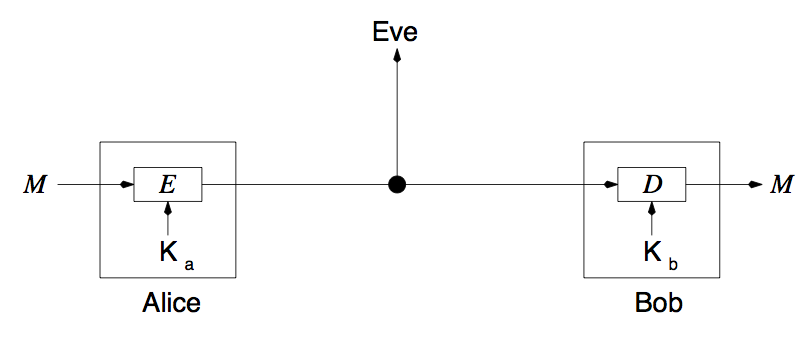
\includegraphics[scale=.25]{./images/traditional_model.png}
  \caption{Traditional Model of Cryptography}
  \label{fig:top_arch}
\end{figure}

\subsection{Side Channel Attacks}
Traditional attacks on cryptographic algorithms use only the input and output of the algorithm, treating it like a monolithic black box.  However, this does not reflect reality.  Algorithms must be implemented in software and run on hardware, which have various properties that change as a result of the cryptographic algorithm's execution.  Side channel attacks use additional data about the encryption process, obtained via observing these information leaks, to circumvent the computational complexity of reversing encryption.  Depending on the algorithm and its implementation, a wide variety of information leaks may exist on a number of different physical channels.  To access and use this leaked information can be very easy or very difficult depending on which channel one is attempting to exploit; for example, getting timing information for a timing attack is as simple as determining the latency between request and response, whereas a power attack requires the attacker to physically access the target system.
%I think the above works better than:
%The attacks which exploit these channels differ greatly in the difficulty of implementation (or the information is easier or harder to get), ranging from utterly simple in the case of timing attacks to requiring physical access in the case of power attacks.
\begin{figure}[ht]
  \centering
  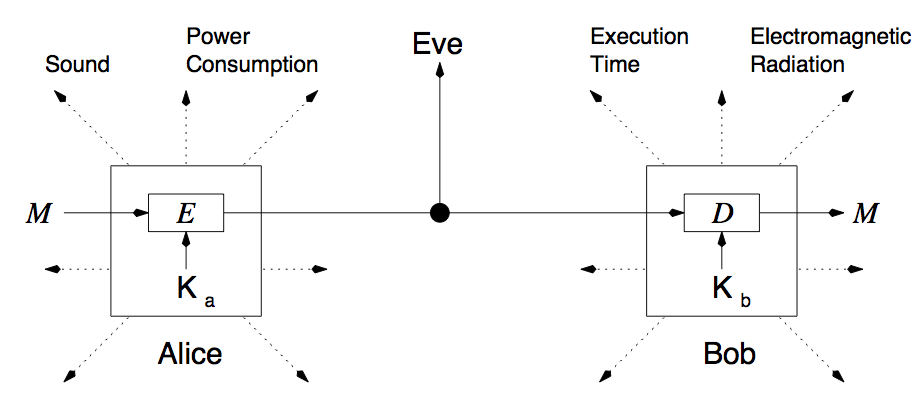
\includegraphics[scale=.25]{./images/side_channel_model.png}
  \caption{Model of Cryptography with Side Channels}
  \label{fig:top_arch}
\end{figure}

\subsubsection{Timing Attacks}
Timing attacks observe variation in the time spent by an encryption algorithm, often with a known input, and use this information to deduce the key.  These attacks generally require a source of feedback on the accuracy of the estimations of the key, which may be gained by submitting multiple requests. These timing data are often compared to a duplicate of the encrypting hardware belonging to the attacker over various keys, enabling better feedback.  Vulnerability to this attack depends on the software implementation of the algorithm, but is rather widespread due to the general drive toward fast algorithms.  The obvious countermeasure is to make the algorithm execute in the same amount of time for any input, but this is difficult due to the unpredictability of compiler optimizations, instruction timings, memory accesses, and so on.  A more useful solution is to obscure the inputs to a vulnerable operation via message blinding\cite{mmthesis}; in RSA this is possible by creating a random pair $(v_{i},v_{f})$ where $v_{f}^{-1}=v_{i}^e$, $e$ being the public exponent, then running the modular exponentiation on $M\cdot v_{i}$ mod $N$ and returning the output multiplied by $v_{f}$\cite{Kocher96timingattacks}. This solution however creates overhead, because now every encryption or decryption requires an extra multiplication step. 

\subsubsection{Caching Attacks}
Caching attacks use a spy thread running concurrently with the encryption program on the target hardware.  The spy thread constantly accesses memory to occupy all lines in the cache, and detects the encryption thread's memory accesses by timing the return of the data; if the encryption thread has evicted the spy thread's cache line for its own use, the spy thread's load operation will take longer.  For some algorithms, such as AES\cite{2004-bernstein-cachetiming}, this enables information about the key (which has precomputed components) to be obtained directly; for others, such as some RSA implementations\cite{Percival05cachemissing}, the program detectably accesses different workspaces in memory due to control flow based on key bits.  These attacks can be partially handled by security-aware thread scheduling and totally prevented by reworking the algorithm to execute code and access memory independently of the input data and key.  The latter would be a tremendous deviation from standard practice and require the significant reworking or abandonment of many existing algorithms\cite{Percival05cachemissing}; as such, it is rarely pursued.

\subsubsection{Branch Predictor Attacks}
Similar to caching attacks, branch predictor attacks involve a spy program running concurrently with the encryption program.  In this case, the spy thread fills all entries in the branch predictor table by simply executing branching instructions throughout its own program. If the encryption algorithm takes a branch, the corresponding branch predictor entry will be occupied by the encryption algorithm. By counting the CPU cycles required to execute a branch, the spy program detects any change in the state of the branch predictor and therefore infers the control flow of the encryption thread, revealing information about the key.  For some algorithms, this attack is capable of obtaining the entire key after spying on only a single encryption operation\cite{branchpredict}.  This attack can be prevented simply by never using secret information to determine a branch, for example through clever use of arithmetic in lieu of conditionals.  This is similar in concept to the dramatic reworking suggested to prevent caching attacks, and thus is not often practiced.

\subsubsection{Power Attacks}
Power attacks use the changing power consumption of the processor to infer the activity of the encryption software over time.  Differences in algorithm activity based on the key will be revealed by the fluctuations they create in processor energy use.  Power attacks require measurement of the power intake of the processor, and are thus generally impossible without physical access to the target hardware, but this is no obstacle in cases such as consumer electronics.  Countermeasures to this sort of attack can be placed in software or hardware; software-based approaches include unconditional execution of operations with large power characteristics, operating on pieces of the secret at a time, and interleaving random computations with the sensitive operations.  Hardware approaches include randomized clocking, power filtering, and power buffering.  Hardware is more expensive to secure than software, but may be necessary depending on the level of security required.\cite{mmthesis}


\section{Elimination of Side Channel Attacks}
We can see a pattern in all of the side channel attacks mentioned above. The attacker collects information from the implementation on the underlying hardware, and use it to infer information regarding the encryption algorithm, which can lead to exposure of the secret key. The branch predictor side channel attack and cache side channel attack both attack a single shared resource from the hardware. By writing a spy process to hog up that resource, an attacker can easily monitor another thread's access to the same resource and therefore monitor the activity of the thread. The timing side channel attack exploits the algorithm's uncontrollable execution time on the processor, and predicts the execution flow to obtain the encryption key. Several individual methods have been proposed to counter the attacks, but they don't tackle the principle cause of the vulnerability -- the uncontrollable and unpredictable execution of software on modern computer architectures. Lickly and Liu~\cite{pret_cases08} introduced PRET (PREcision Timed Architecture), an architecture that delivers predictable timing along with predictable function and performance. This architecture tackles the root cause of side channel attacks by design, eliminating the vulnerability.

We present an overview of the PRET architecture in the context of eliminating side channels attacks, and refer interested users to ~\cite{pret_cases08} for more details. We assume the reader has a basic understanding of computer architecture, such as how pipelining and caches work. Readers that aren't familiar with these terms are advised to see \cite{patterson2005coa} for an introduction.

%\begin{wrapfigure}{r}{0pt}
%  \end{wrapfigure}
\subsection{PRET Architecture}

\begin{figure}[ht]
  \centering
  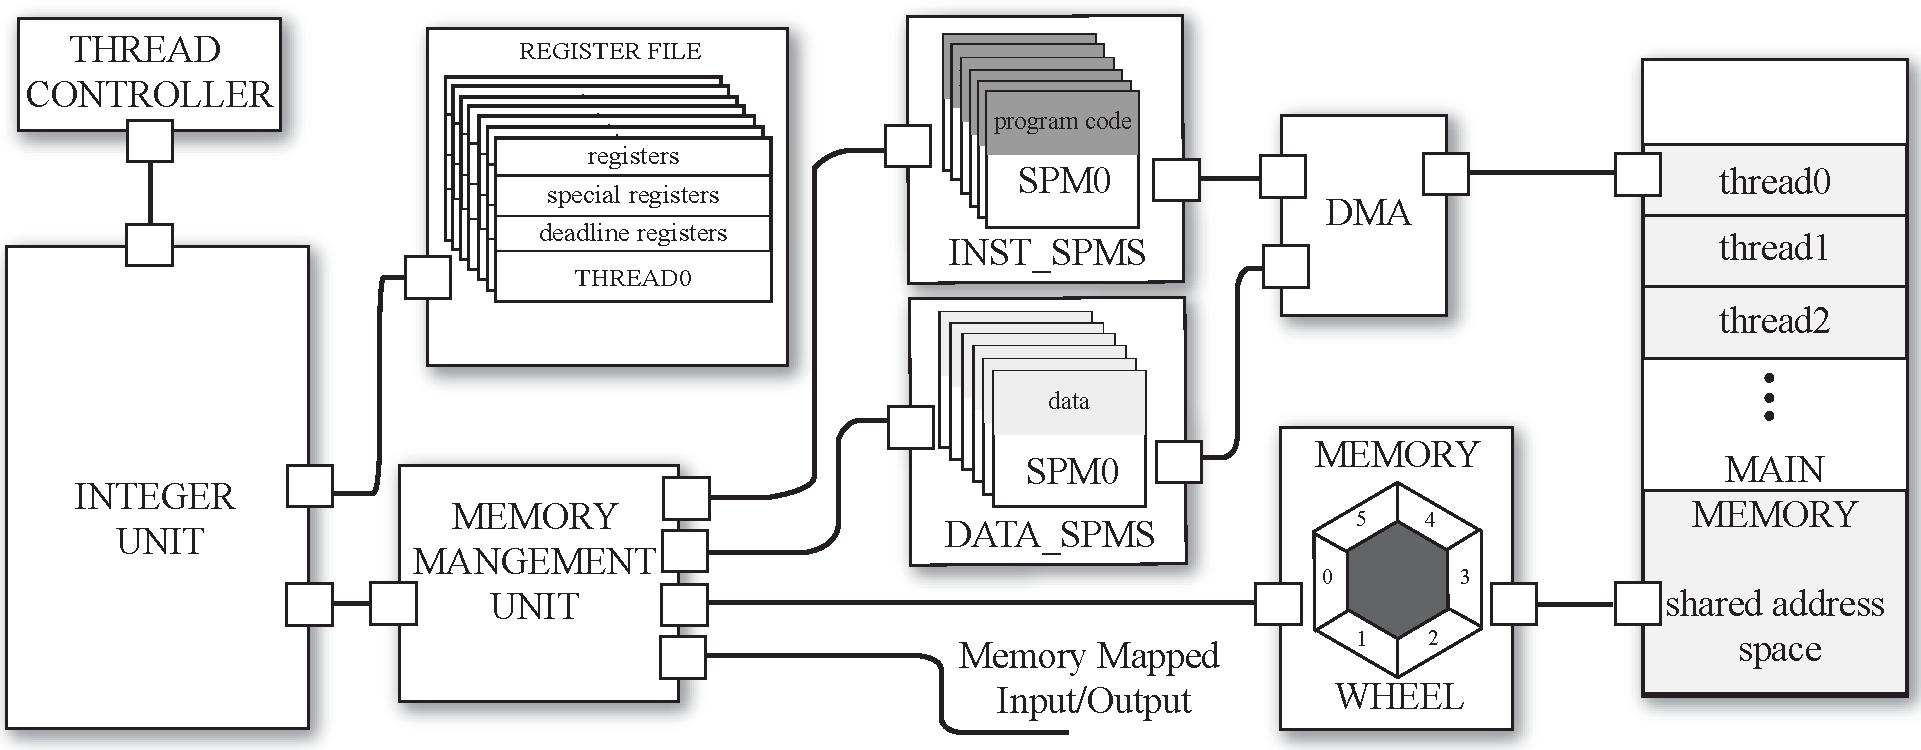
\includegraphics[scale=.25]{./images/top_arch.pdf}
  \caption{Block Diagram of PRET Architecture}
  \label{fig:top_arch}
\end{figure}

A block level diagram of the PRET architecture is shown in Figure~\ref{fig:top_arch}. The core integer unit pipeline of the PRET architecture implements a thread-interleaved pipeline. Hardware units that keep the processor's state such as register files or local on-chip memories are duplicated for each hardware thread to keep each thread independent. Threads are scheduled to execute in a predictable round-robin fashion. Scratchpad memories (SPM)\cite{Banakar2002} are employed instead of caches to allow controlled and predictable access to local on-chip memories. A memory controller facilitates time-triggered access to the off-chip main memory through a memory wheel to decouple the threads' access to memory from each other. In addition, ISA support is provided to bring timing semantics to the software level.

\subsubsection {Thread-Interleaved Pipeline}
Pipeline hazards occur because the next instruction to be fed into the pipeline does not have the required information to be executed. Conditional branches are the prime example -- the pipeline cannot fetch and execute the next instruction without knowing what it is. The penalty of hazards can be mitigated by introducing hardware units that speculate the next state; branch predictors speculate the next instruction, and caches speculate the data that will be accessed in the near future. If the speculation is correct, there is no penalty and the processor continues to execute. But if it is incorrect, then the processor must do extra work to recover by discarding the speculated work and re-executing the correct instructions. These mechanisms are the main cause of unpredictable execution time because in software there is no way of knowing whether the hardware speculation is correct or not. 

If we can remove pipelining hazards, then we can remove the need for the speculation units. Lee~\cite{lee1987pipeline1} proposed using thread interleaved pipelines to remove data dependencies and control hazards in the pipeline to get predictable and repeatable behavior. The basic idea is shown in Figure \ref{fig:int_pipe}. 
\begin{figure}[ht]
  \centering
  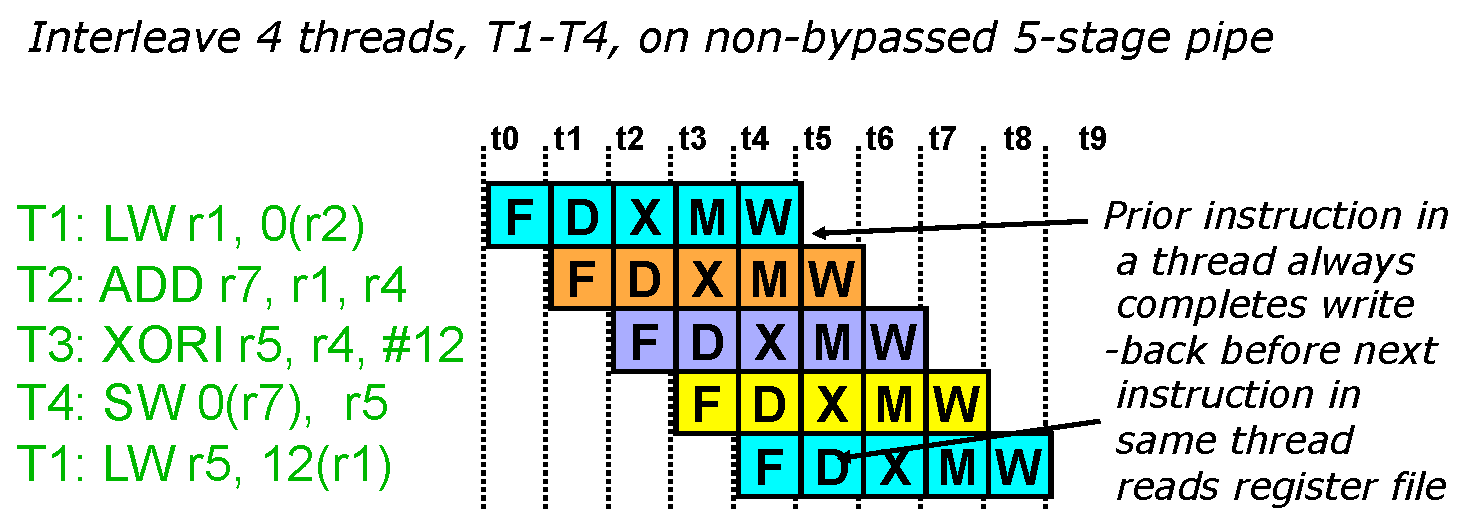
\includegraphics[scale=.35]{./images/interleavedpipeline.pdf}
  \caption{How interleaved threading removes data dependencies}
  \label{fig:int_pipe}
\end{figure}

Via thread-interleaving, we can completely remove any data forwarding logic in the processor, along with the branch predictors, because we have no need to speculate the next instruction to be executed. Simply by focusing on repeatable and predictable behavior in the design of the pipeline, we have removed the vulnerability that enabled the branch predictor attack. 

\subsubsection {Memory System}
Fast access on-chip memory is a requirement for modern processors. The high clock speed of the processor combined with the high latency of main memory results in hundreds of cycles lost when the processor needs to access the off-chip main memory. Caches are a hardware controlled fast access memory that tries to predict and pre-fetch the data from main memory for the processor based on temporal and spatial locality of data access. If the cache control speculation is accurate, then access to data can complete in one cycle of the processor. However, if a misprediction occurs, the time it takes to access the data is drastically longer. Thus, cache hits and misses often determine the performance of a program, cause it to be the major source of timing unpredictability~\cite{thiele:04:predictable}.

Unlike the branch predictor, removing fast access memories is not an option, since it will result in a huge performance overhead. Instead, we use scratchpad memories as an alternative to caches. Scratchpad memory brings the control over the fast access memory to software. The compiler can pre-allocate the data locations in the fast access memory, resulting in predictable performance (since we always know which accesses are hits or misses). The software may also control the loading of scratchpad memories at run time by using Direct Memory Access instructions without a loss of predictability. Ongoing research has shown methods to efficiently manage the scratchpads~\cite{avissar2002oma, Bandyopadhyay:EECS-2006-105, Patel:EECS-2008-115} to optimize the performance of a program, but that is  beyond the scope of this paper. 

Unlike on simultaneous multi-threaded architectures, a cross-hardware-thread cache side channel attack is not possible because each thread has its own separate physical scratchpad memory. Only if multiple software threads were to run on a single hardware thread, then two software threads would share the same scratchpad. However, because the allocation of memory on the scratchpad is software controlled, any underlying software thread supervisor would have complete control over the scratchpad allocation. One could imagine a management scheme similar to virtual memory for scratchpads to separate access for each thread. Again, by designing the architecture to preserve predictable and repeatable timing, we have removed the vulnerability that enables caching attacks.

\subsubsection {Instruction Set Architecture Extension}
Even with a timing-predictable architecture that executes instructions in a deterministic way, algorithms and programs naturally introduce varying run times because each iteration may follow a different path in the code. Clever Instruction Set Architecture (ISA) designs have bridged the developer and the machine extremely well, providing simple enough instructions for the machine to be kept simple, and yet still provide expressability to the programmer. However, this level of abstraction has failed to bring temporal semantics of the underlying architecture up to the software level. One way to control execution time is through programming external timers and interrupts, which the hardware must support. This is both tedious and difficult to program, and the resulting code is non-portable. 

Ip and Edwards~\cite{ip2006processor} propose a processor extension that allow explicit timing control at the ISA level. They introduce deadline registers which are decremented each clock cycle if it contains a value other than zero. Deadline instructions load values in the deadline register when the register is zero. A basic example is shown in figure~\ref{fig:deadline}.

\begin{SCfigure}
  \centering
  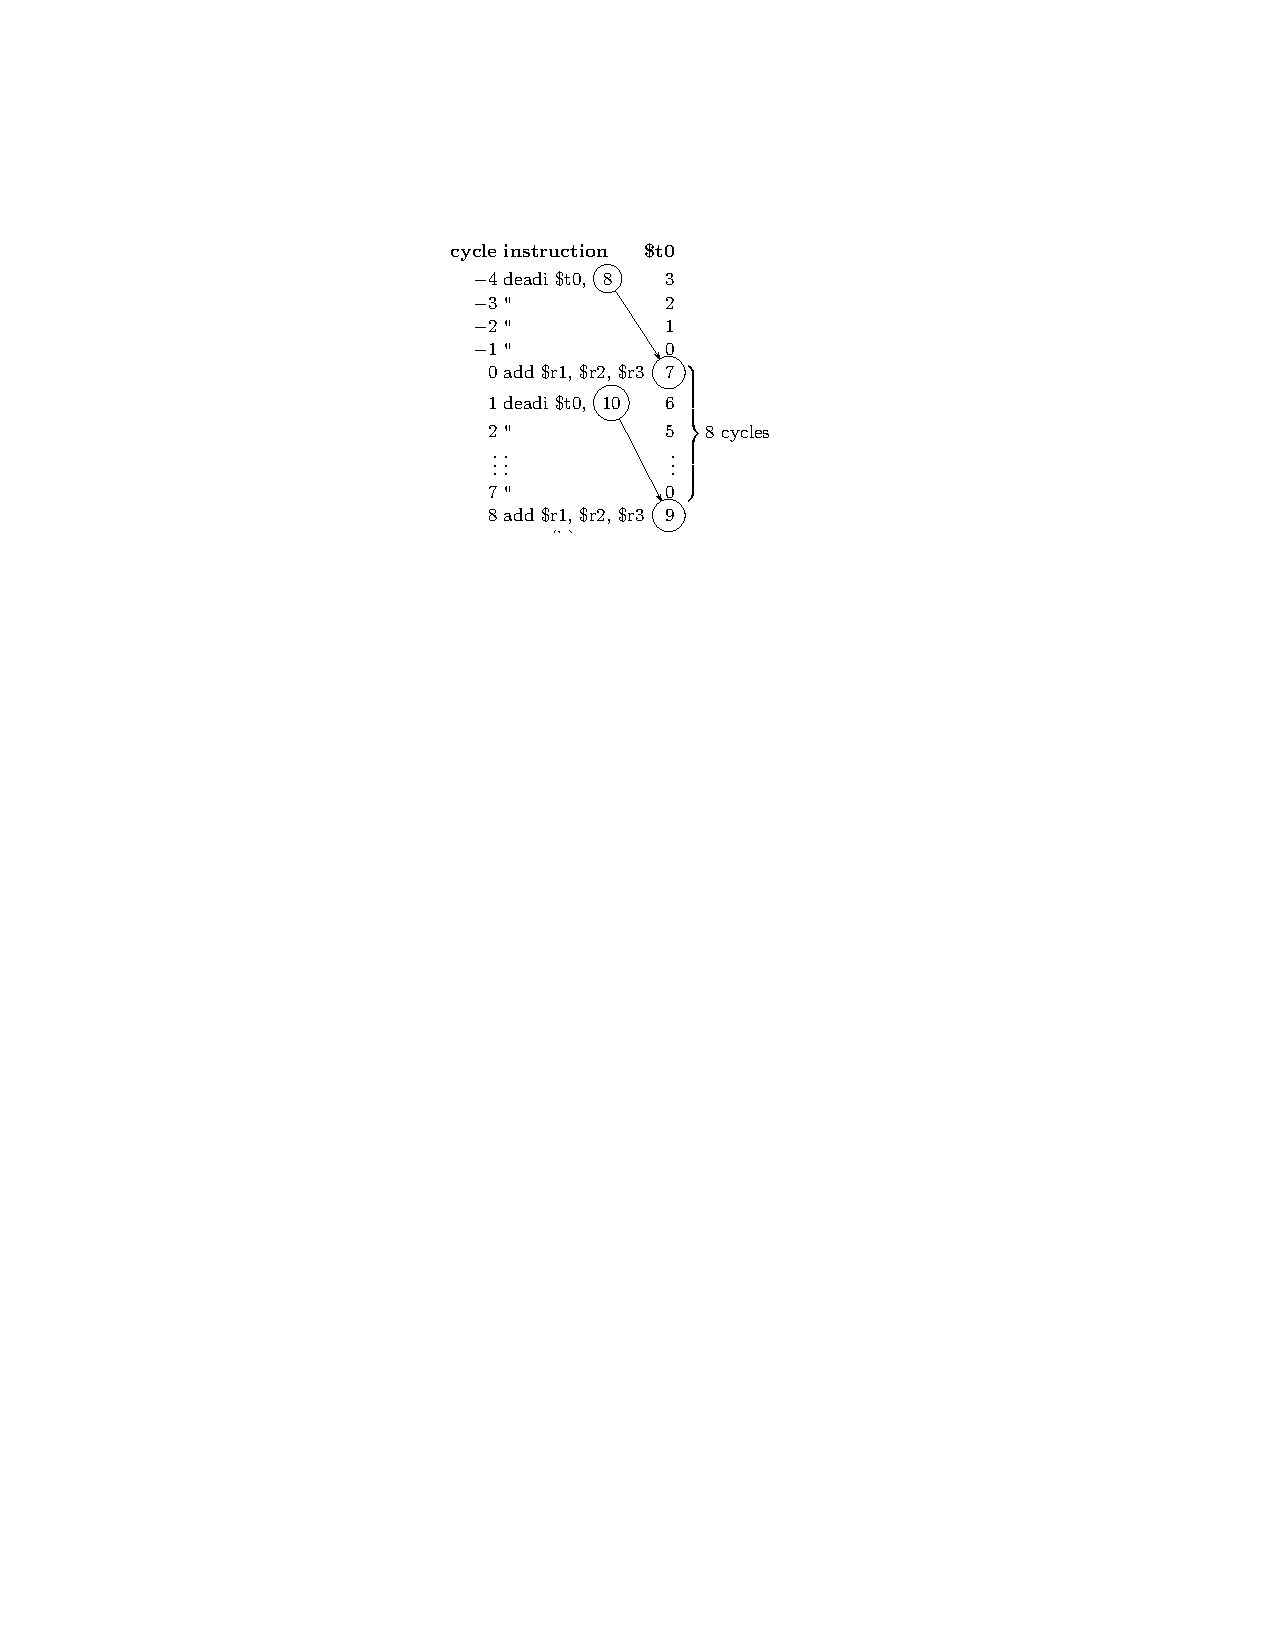
\includegraphics[scale=.85]{./images/deadlineExp.pdf}
  \caption{By enclosing the add instruction with deadlines, we ensure that the 2 adds are executed 8 cycles apart. \$t0 is a deadline register. When a deadline instruction is encountered, the program does not progress forward until the deadline register is decremented to 0.}
  \label{fig:deadline}
\end{SCfigure}

This allows control over execution time of the program at the software level, without dealing with interrupts and external timers. This extension along with a predictable architecture allow programmers full control over the run time of a program, allowing them to write predictable and precision timed code and defend against timing side channel attacks. 

\section{Case Study}
\subsection{RSA Vulnerability}
The central computation of the RSA algorithm is based primarily around modular exponentiation.  It takes the form 

\begin{center}\fbox{\parbox{6cm}{INPUT: M, N, d = $(d_{n-1}d_{n-2} . . . d_{1}d_{0})_{2}$ 
OUTPUT: S = M$^{d}$ mod N 

\hspace{2mm}S $\leftarrow$ 1 

\hspace{2mm}for j = n - 1 $. . .$ 0 do 

\hspace{4mm}S $\leftarrow$ S$^{2}$ mod N

\hspace{4mm}if d$_{j}$ = 1 then 

\hspace{6mm}S $\leftarrow$ S $\cdot$ M mod N 

\hspace{2mm}return S 
}}\end{center}

Paul Kocher outlined\cite{Kocher96timingattacks} a notional side-channel timing attack on this algorithm that requires a large number of plaintext-cyphertext pairs and detailed knowledge of the target implementation.  By simulating the target system for predicted keys, the actual key could be derived one bit at a time.  An improved method \cite{DKLMQW98} demonstrated the ability to obtain even a 512-bit key in a reasonable amount of time.  Our analysis of the algorithm demonstrated that a significant portion of the variation in the algorithm's execution time could be attributed to the branch in the loop above.  When the reference implementation of RSA (RSAREF 2.0) was ported to the PRET architecture, single iterations of the loop varied in execution time almost exclusively due to the value of d$_{j}$.  As seen in Figure \ref{fig:modexp}, each iteration took approximately either 440 or 660 kilocycles, with very little deviation from the two means.  This is far more than sufficient for a successful timing attack; 0.2\% of that difference was adequate in one case! \cite{DKLMQW98}

\begin{figure}[ht]
  \centering
  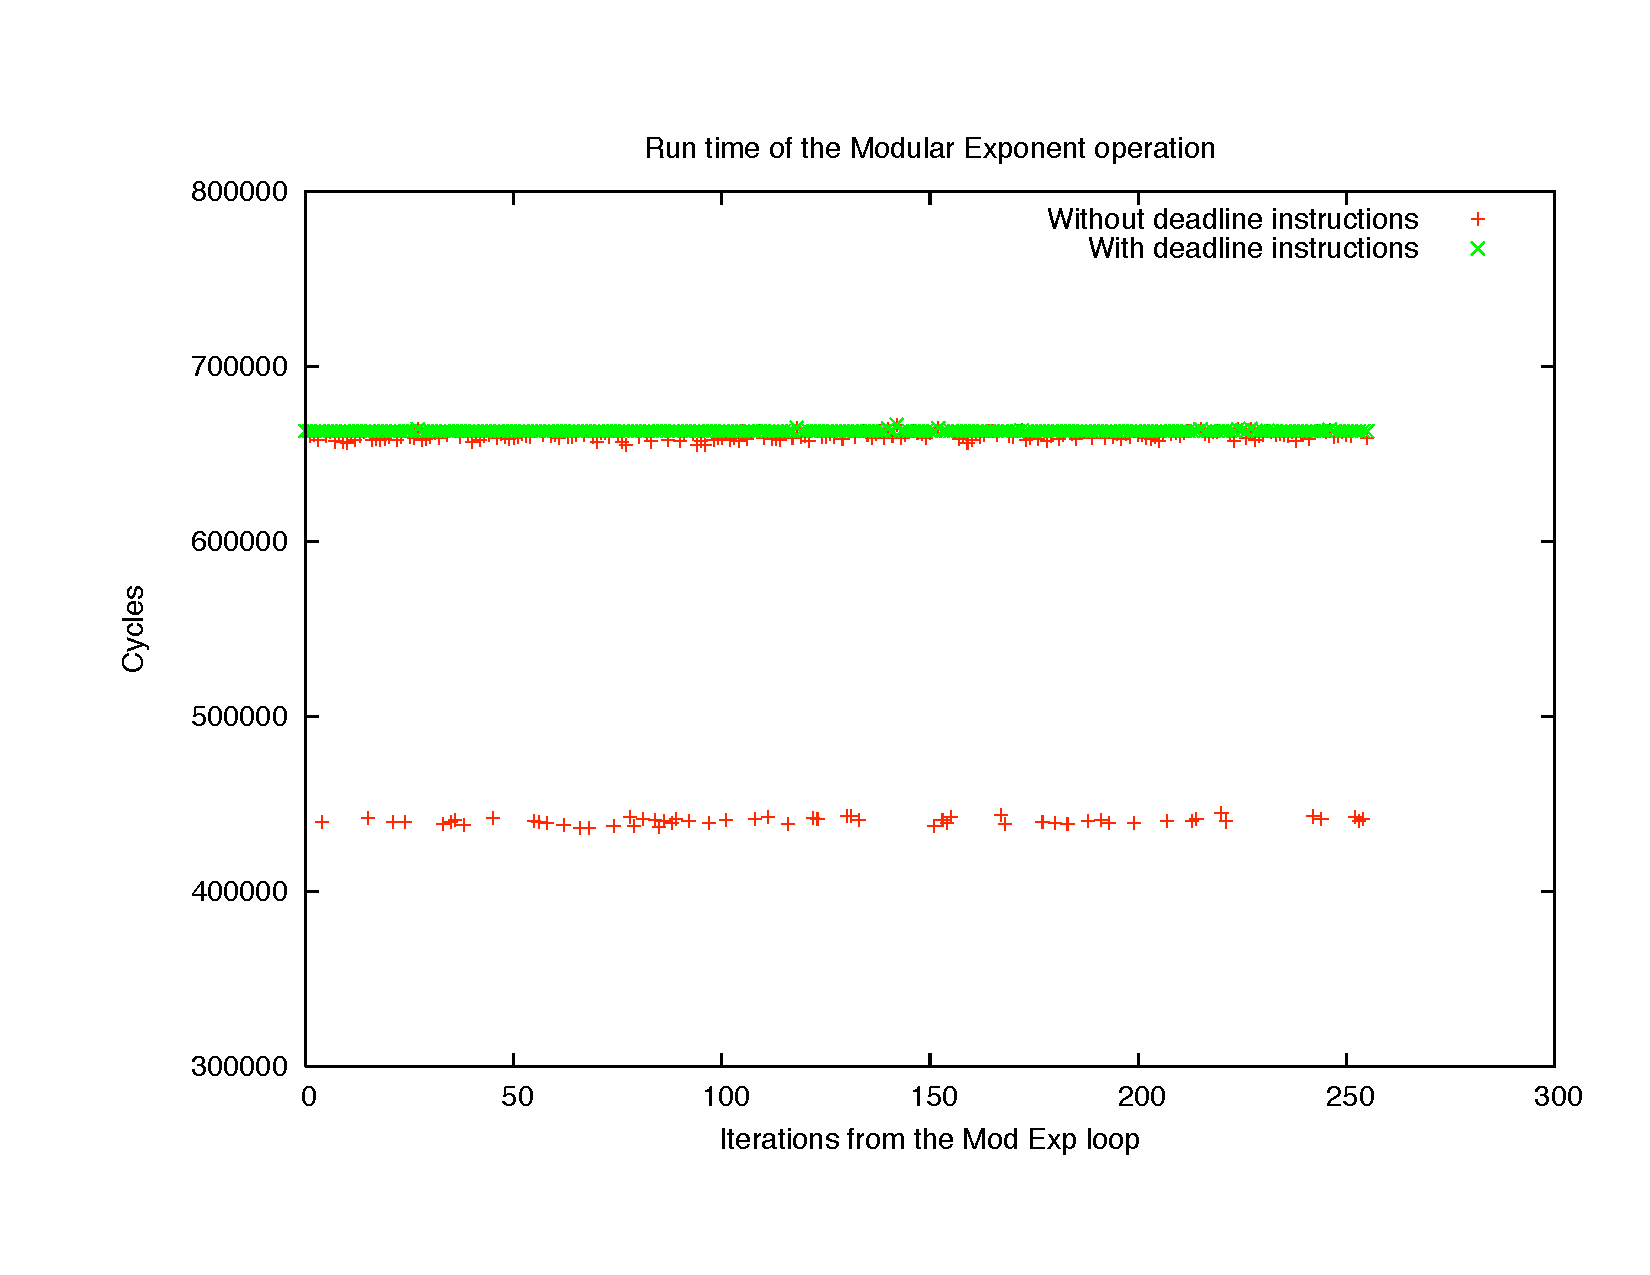
\includegraphics[scale=.3]{./images/ModExp.pdf}
  \caption{Run time of Modular Exponent operation}
  \label{fig:modexp}
\end{figure}

\subsection{Removing the Vulnerability}
By simply adding a PRET deadline statement in the body of the loop, the bimodality of the execution time is totally eliminated, as seen in Figure \ref{fig:modexp}.  As enforced by the deadline, all iterations take the same amount of time.  Additionally, placing a deadline on this loop eliminates the vast majority of the variation in the runtime of the entire program.  Figure \ref{fig:rsa} shows the large-scale effect:  Without the deadline, different keys exhibit significant diversity in algorithm execution time.  When the deadline is added, the fluctuation is dramatically reduced, and what variations from the mean exist are not even obviously correlated to the variations that existed before.  This indicates that the much smaller abnormalities that have been revealed stem from a different source.  The algorithm contains other branches that affect runtime, but evidently none so significant as the one in the loop which was made irrelevant by the deadline. It is obvious at this point that we could simply do a worst case execution time analysis, and enclose the entire encryption algorithm within one deadline instruction. This effectively removes even the remaining fluctuations and will cause the encryption to ALWAYS run in the exact amount of time.

\begin{figure}[ht]
  \centering
  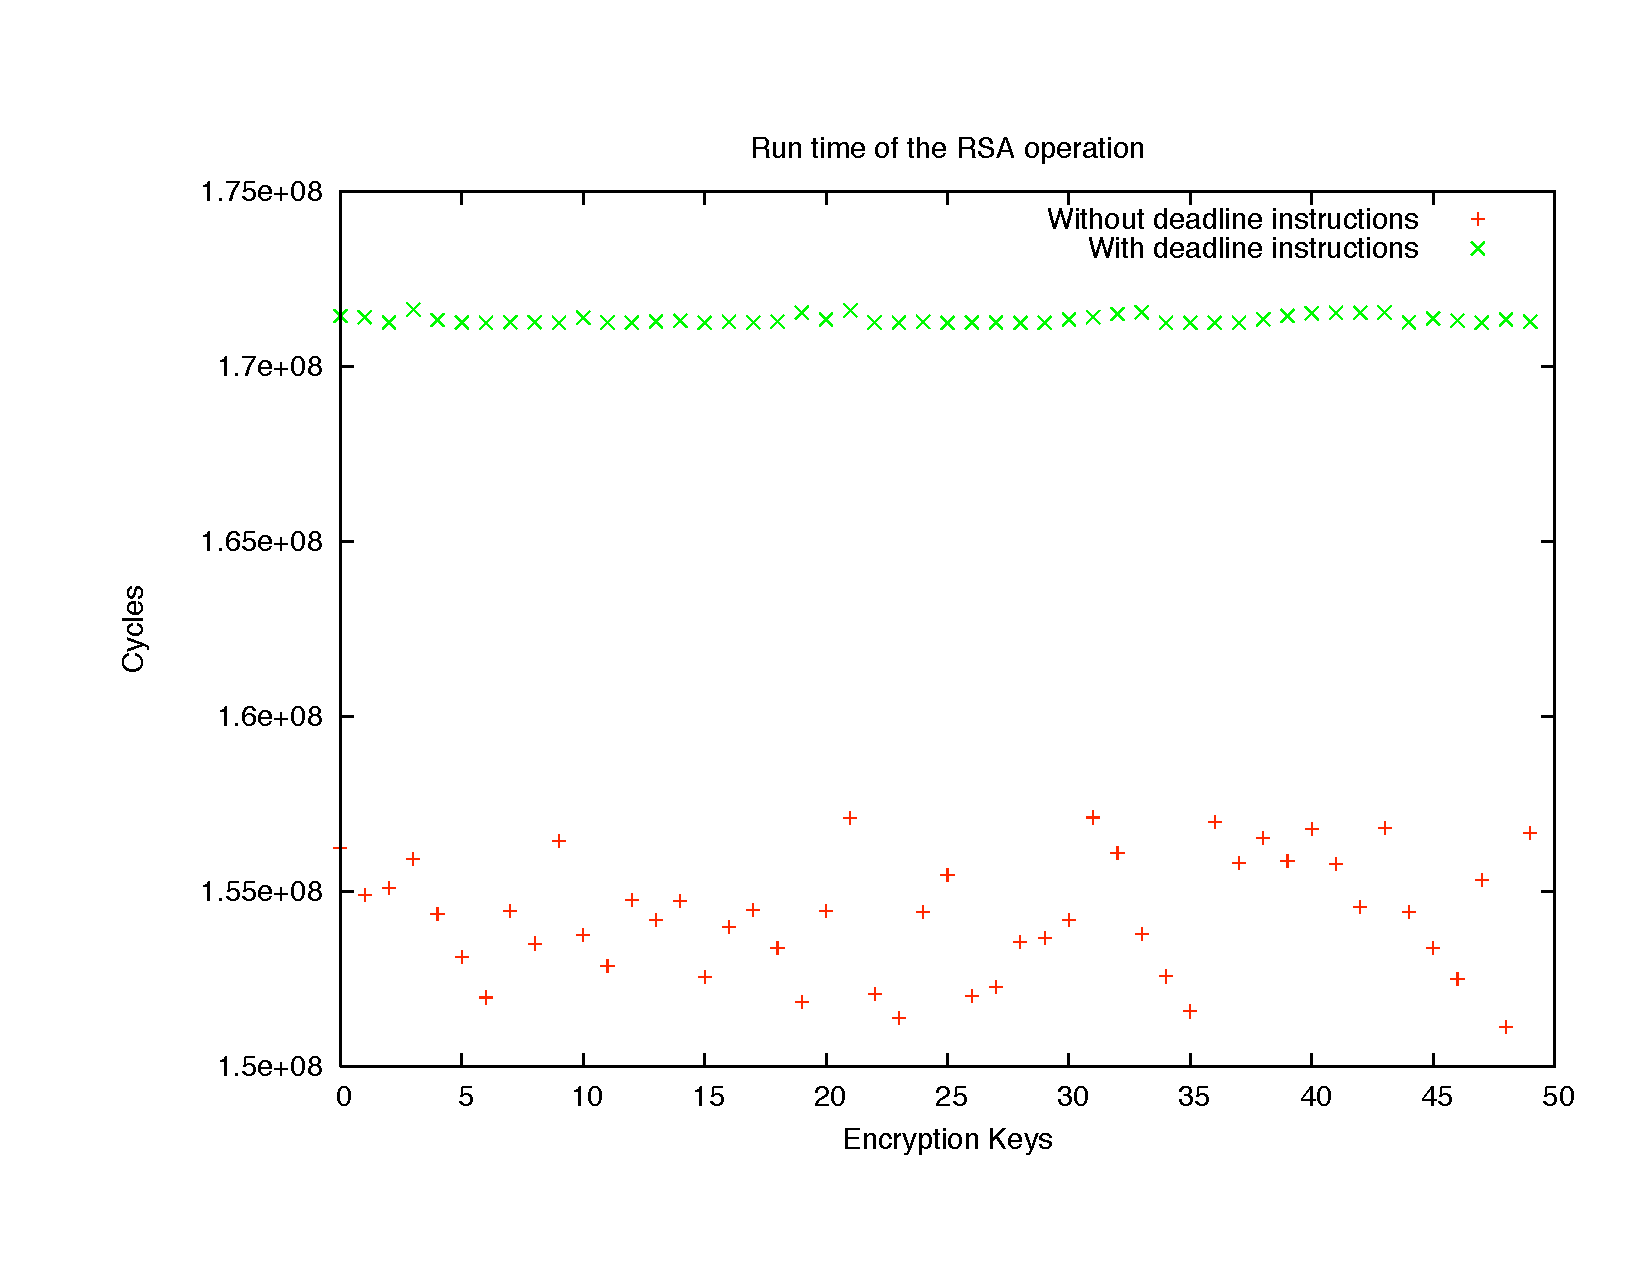
\includegraphics[scale=.3]{./images/RSA.pdf}
  \caption{Run time of RSA operation}
  \label{fig:rsa}
\end{figure}

In addition to its resistance to timing attacks, simply by running on the PRET architecture, this RSA implementation is now immune to cache attacks and branch predictor attacks, both of which can be significant dangers to RSA\cite{branchpredict, Percival05cachemissing}.

\subsection{Remaining Vulnerabilities}
PRET was designed to tackle temporal unpredictabilities in the architecture. Since the current implementation is a software simulator, we cannot evaluate the power vulnerabilities. It might be the case that the processor will consume less power while waiting for the deadline register to count down. As a result, measuring power consumption instead of time elapsed might still reveal variations very similar to those observed in execution time when there were no deadlines.  Depending on the application's demands, this may be acceptable.  However, power attacks could also be prevented with additional architecture features; as the PRET architecture is intended for real-time applications rather than security applications, it is not designed to burn power while waiting, but such functionality could be added and controlled in software by processor state registers to allow a power burning mode while doing the encryption, and a switch back to power saving mode when not.  

\section{Conclusion}
Side-channel attacks are a credible threat to many cryptographic systems.  Their capability derives not from a weakness in an algorithm's mathematical underpinnings but from information leaks in the implementation of the algorithm.  Without secure hardware, software cannot be considered truly secure.  Some stopgap measures are implementable in software, but rarely are they a guaranteed fix.

In this paper we lay out a means of attacking the root cause of side-channel attacks - the means of information leakage.  By securing the hardware element via an architecture founded on predictable performance, we allow a slightly modified encryption algorithm to entirely resist timing, cache, and branch prediction attacks.  Judicious use of deadline instructions to hide branch-induced runtime variations prevent timing attacks, the presence of thread-specific scratchpad memory instead of shared cache makes cache attacks impossible, and the absence of any need for a branch predictor likewise rules out branch predictor attacks.

We demonstrate the application of these principles to a known-vulnerable implementation of RSA.  In an unmodified state on secure hardware, it has significant runtime variations that can be used to derive the private encryption key.  When modified to take advantage of the timing-invariance features of the hardware, its increased resistance to timing attacks is obvious.  Other algorithms which require security could be similarly ported to security-enabling hardware and easily modified to become immune to a number of dangerous side-channel attacks.

\bibliographystyle{latex8}
\bibliography{RTencryption}

%-------------------------------------------------------------------------

\end{document}
